We have presented a method of nonlinear dimensionality reduction that is compatible with the scale and composition of modern biobanks. With UMAP and HDBSCAN($\hat{\epsilon}$) we have uncovered a wide variety of patterns of fine-scale population structure in every biobank studied. Since the publication of \hyperref[chap:chapter1]{Chapter~1} , UMAP has become a standard method for visualization and exploratory data analysis in population genetics. Given the demand for cluster extraction noted in \hyperref[chap:chapter3]{Chapter~3}, it is possible that HDBSCAN($\hat{\epsilon}$)---or some other density clustering method---could see similar adoption.

The timing of UMAP coincides fortuitously with the growth of biobanks and the genomic revolution. Writing in his review of TDA in 2018, Wasserman asked, ``is it possible to derive low dimensional embedding methods that explicitly preserve topological features of the data? This is an interesting open question.''\citep{wasserman_topological_2018} This review was published in the same year that UMAP, an explicitly topological method, was released. Topological analysis and density clustering seem especially well-suited to the task of understanding population structure in diverse biobanks.

\section{The value of visualization}

In \hyperref[chap:chapter2]{Chapter~2} we describe the relationship between dimensionality reduction and biological data as analogous to that of microscopes and biological samples. This analogy has been made before with respect to mathematics in general\citep{cohen_mathematics_2004}. Though analyses, inferences, and models can shed light on the biological world, there is an inherent value to being able to literally see your data and understand its structure. Among the most cited papers in population genetics is ``Genes mirror geography within Europe''\citep{novembre2008europe}---although isolation-by-distance had been characterized almost a century earlier, the figure of the top principal components superimposed over Europe was an elegant illustration of the geographical distribution of human genetic variation.

With UMAP, we are able to map complex genetic structure down to $2$ or $3$ dimensions for visualization, examine the fine-scale structure that a method like PCA compresses, while preserving interesting signal in the data. Using auxiliary data---geographic data, population labels, phenotypic information, environmental variables, etc.---we can visually scan for patterns and generate hypotheses. In \hyperref[chap:chapter1]{Chapter~1} we present a variety of visualization methods, including using colouring points by admixture levels to uncover gradients in ancestry and converting 3D UMAP coordinates to RGB colour levels for colouring maps. One common method used in single-cell studies is to colour UMAP plots by gene expression levels (e.g. \citep{jessa_stalled_2019} Figure~4h). A similar approach could be used in exploring allele distributions by clusters to see whether they are relatively more common in different populations---one such method, called the Allele Dispersion Score, was proposed by Correard et al. in 2022\citep{correard_allele_2022}. Though UMAP figures are now standard in genetic studies, most are limited to a simple 2D scatterplot coloured by some population label---in every biobank, there is certainly value in exploring deeper and using other variables.

There is also value in going beyond static $2$D figures. Software libraries such as plotly\citep{plotly} can generate interactive figures, are available for Python and R, and are straightforward to implement. Interactive exploration can assess how individual points fit within larger projections, rapidly identifying patterns or using them for diagnostics. Working in $3$D is much easier when the figures are interactive, and we have found value in, e.g., exploring the relationships between individuals and populations in the UKB. Finally, as noted in \hyperref[chap:chapter3]{Chapter~3}, clustering works well in dimensions abvoe $2$---while it can be tempting to delineate clusters from $2$D figures alone, the jump from $3$ to $2$ dimensions can lose information about how points are related to one another topologically. There is value in using information from higher dimensions to aid visualization in lower dimensions and, despite UMAP's now-widespread use, its ability to work in $3$ or more dimensions is, in the view of the author, underappreciated.

\section{Clustering in human genetics}

Unlike problems like classification, clustering does not have a well-defined ground truth, and even the most basic definition, such as ``similar points are grouped together and dissimilar points are grouped separately'', can be self-contradictory\citep{ben-david_clustering_2018}. In a genetic cluster from \hyperref[chap:chapter3]{Chapter~3}, individuals in may be closely related to their immediate neighbours, but not to those in a far end of a cluster; they are grouped by similarity in one sense, but not separated by dissimilarity. Different algorithms and parametrizations will yield different results. Though various quality metrics exist, it has been argued that even untrained humans are better at assessing the quality of an arbitrary $2$D clustering\citep{lewis_human_2012}---there is an element of ``I know it when I see it''. 

The question of the appropriateness of a given clustering can be framed as whether it is useful in its context: whether it helps to find interesting patterns (without necessarily assigning interpretation); whether it simplifies data; investigation correlations with other variables, etc\citep{hennig_what_2015}. The choice of clustering method is often arbitrary, e.g. ``we use the standard method in the field''\citep{ben-david_clustering_2018}, and this has resulted in standards that exclude individuals from analyses\citep{ding_polygenic_2023}. We have demonstrated that density clustering successfully includes all or almost all individuals in several biobanks and that the clusters generated reflect logical groupings.
\citep{hennig_what_2015}

There are no ``true'' clusters; the idea of ``underlying truth'' or ``natural kinds''


One of the questions around clustering is whether we have found ``true clusters''; that is, whether they reflect some ``truth''. 

It is better to gauge clusters by how useful they are and what they may reflect rather than representing something concrete and tangible. Clusters matching population labels in the 1KGP signified not that the populations were ``real'', but that the algorithm successfully capture the source of structure in the data---i.e. the sampling scheme.

``Empirical'' is not the same as ``objective''

\citep{lewis_human_2012}

This is a question of epistemology---

There is no universal definition of a ``cluster'', and the idea of a ``good'' clustering will be domain-specific\citep{hennig_what_2015}.

- discrete groupings are useful, like models --- and like models, they are prone to reification: the territory is not the map
- the philosophy of unsupervised learning and clustering in general
- we're finding something, it's probably not nothing


\clearpage

\section{Defining populations}

\begin{figure}[h]
\centering
\begin{subfigure}{0.45\linewidth}
    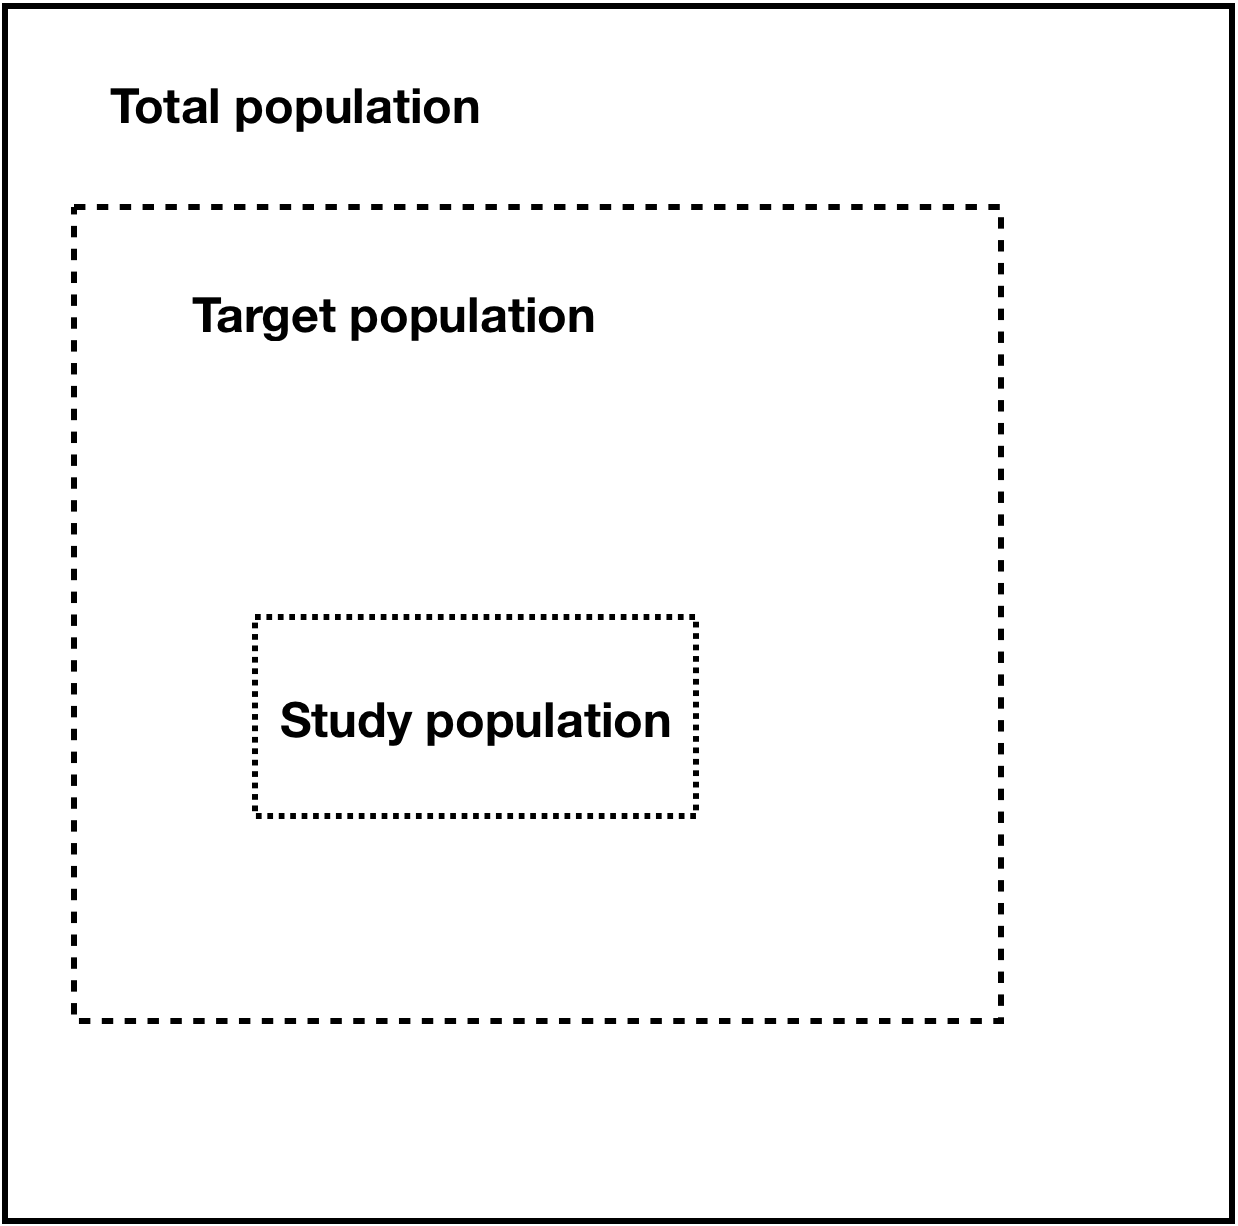
\includegraphics[width=\linewidth]{main_figures/discussion/populations_1.png}
    \caption{}
    \label{fig:statistical_populations1}
\end{subfigure}
\hfill
\begin{subfigure}{0.45\linewidth}
    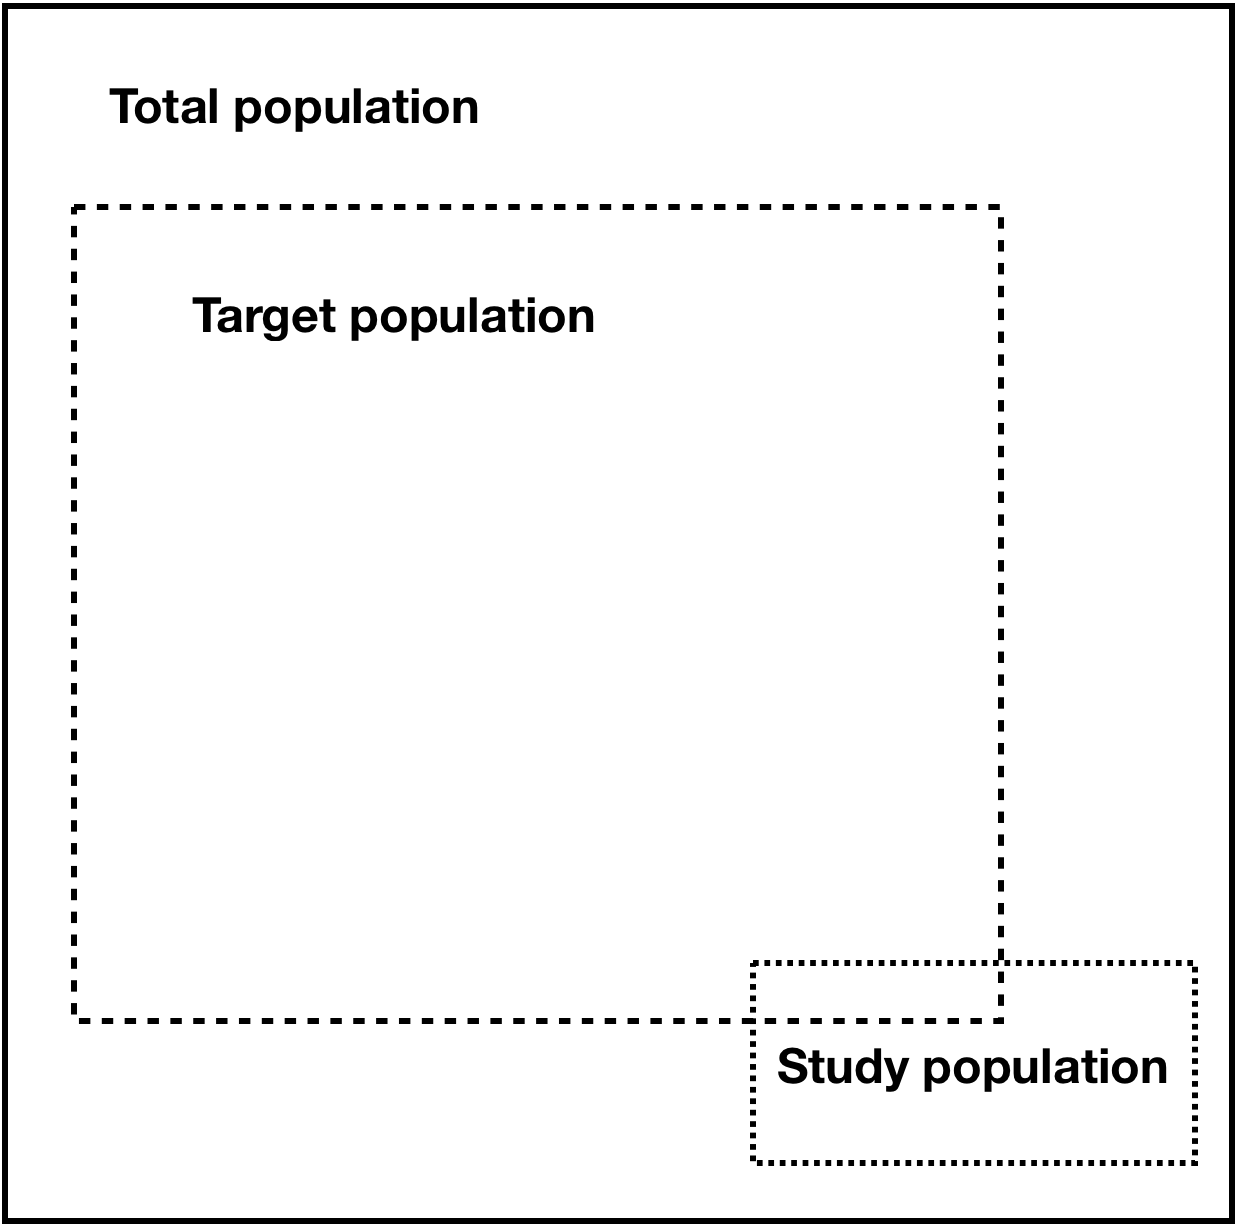
\includegraphics[width=\linewidth]{main_figures/discussion/populations_2.png}
    \caption{}
    \label{fig:statistical_populations2}
\end{subfigure}
\caption[The relationship between target and study populations]{\textbf{The study population should match the target population.} In \textbf{(a)}, the study population is a subset of the target population, so inferences drawn from it will apply to the target population. In \textbf{(b)}, the study population is not fully a subset of the target population, so its inferences will be less reliable.}
\label{fig:statistical_populations}
\end{figure}

Though genetic variation exists on a multidimensional continuum, defining discrete populations can be useful, e.g. for modelling ancestry\citep{pritchard_inference_2000}. In inferential statistics, we also require a definition of ``population''\citep{statcan2003}. To establish the scope of a study, we define the ``target population'' (the group to which research applies) and the ``survey population'' (the group which is covered by the study and, ideally, is very similar to the target population). The survey population is ultimately chosen from the survey frame, which provides the means to sample the individuals from the population. Figure~\ref{fig:statistical_populations} provides a schematic of this concept, as well as a schematic of when the study population is not drawn from the target population.

Pgh1: Biobanks are the sources of biomedical studies, but how do they define their study populations and how do they define their target populations? Also point out that the studies done are not random samples from the target population but volunteer-based non-random samples. Then mention some of the associates found between markers and participationi n the UKB.

Pgh2: The way we define populations is pretty archaic and not great. Segue into hte next section (subsection?) where we discuss the histories of these ideas

Biobanks are the source of many biomedical studies, particularly GWAS and PGS. 

This principle applies to inferences and studies based on biobanks. 

In practice, biobank inference is often based on a form of non-probability sampling. 

-COB, ethnicity, biobank selection and ascertainment bias, etc

[talk about popgen, biobanks, assumptions, etc]


Structure may be subtle and arise from, e.g., recent population structure or admixture\citep{gopalan_human_2022}

Bigger data is not better data. We cannot just collect our way out of this --- we need to understand what it is that we are doing and what we are working with.



Though clustering is often viewed as a statistical or computational method, it has topological underpinnings as well.

genetics of participants may not match non-participants
\citep{benonisdottir_studying_2023}

The UKB's nested structure, and how definitions shape our perceptions.

\subsection{Labels and how data are situated}



\section{Equitability in the genomic revolution}



PRS more like LOL\citep{kaplan_polygenic_2022}

\section{The genetics-environment interplay}

Sick people and sick populations\citep{rose_sick_2001}

Biases in biobanks?

\section{History of the field}

The meanings of structure, biological essentialism, and the shadow of eugenics.

What we show undermines these narratives---there are no true clusers, no true populations, no perfect models or representations, but there are \textit{useful} ones.

Bad actors are not motivated by methodology---the correlation coefficient, the density plot, and the scatter plot remain common tools in spurious claims. Still we must take care in the way we present our research, understanding that it can easily be stripped of context.

Algorithmic colonialism, helicopter/imperialistic research, 

\citep{gebru_race_2020}



\section{Limitations}

\section{Etc}

Biology is the new physics \citep{hunter_biology_2010}
